%!TEX root = ../larxxia.tex


\section{Regularise linear equations}
\label{sec:rle}
\secttoc

\begin{quoted}{\parbox{15em}{Sherlock Holmes, in The Boscombe Valley Mystery, by Sir Arthur Conan Doyle, 1892}}
Singularity is almost invariably a clue.
\end{quoted}


Often we need to approximate matrices involved in solving linear equations.  
This is especially so when the matrix itself comes from experimental measurements and so is subject to errors.
We do not want such errors to affect results.
By avoiding division with small \idx{singular value}s, the procedure developed in this section avoids unwarranted magnification of errors.
Sometimes such error magnification is disastrous, so avoiding it is essential.

\begin{example} \label{eg:2regu}
Suppose from some experiment we to solve the linear equations
\begin{equation*}
0.5x+0.3y=1\quad\text{and}\quad 1.1x+0.7y=2\,,
\end{equation*}
where all the coefficients on \emph{both} the left-hand sides and the right-hand sides are determined from experimental measurements.
In particular, suppose they are measured to errors~\(\pm0.05\)\,.
Solve the equations.
\begin{solution} 
\begin{itemize}
\item Following Procedure~\ref{pro:unisol} in \script, form the matrix and the right-hand side
\begin{verbatim}
A=[0.5 0.3;1.1 0.7]
b=[1.0;2.0]
\end{verbatim}
Then check the condition number with \verb|rcond(A)| to find it is~\(0.007\) which previously we would call only just outside the `good' range (Procedure~\ref{pro:unisol}).
So proceed to compute the solution with~\verb|A\b| to find \((x,y)=(5,-5)\) (as illustrated in the margin).
\marginpar{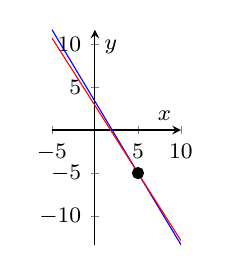
\begin{tikzpicture}
  \begin{axis}[footnotesize,font=\footnotesize ,axis equal image
  , xlabel={$x$}, ylabel={$y$}, axis lines=middle,domain=-5:10
  ]
  \addplot[blue] {(1-0.5*x)/0.3};
  \addplot[red] {(2-1.1*x)/0.7};
  \addplot[black,mark=*] coordinates {(5,-5)};
  \end{axis}
\end{tikzpicture}}

\item Is this solution reasonable?  No.  Not when the matrix itself has errors.
Let's perturb the matrix~\(A\) by amounts consistent with its experimental error of~\(\pm0.05\) and explore the predicted solutions (the first two illustrated):
\marginpar{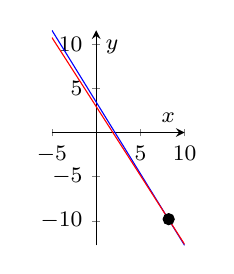
\begin{tikzpicture}
  \begin{axis}[footnotesize,font=\footnotesize ,axis equal image
  , xlabel={$x$}, ylabel={$y$}, axis lines=middle,domain=-5:10
  ]
  \addplot[blue] {(1-0.47*x)/0.29};
  \addplot[red] {(2-1.06*x)/0.68};
  \addplot[black,mark=*] coordinates {(8.2,-9.8)};
  \end{axis}
\end{tikzpicture}}%
\marginpar{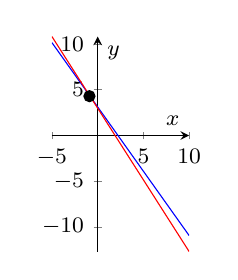
\begin{tikzpicture}
  \begin{axis}[footnotesize,font=\footnotesize ,axis equal image
  , xlabel={$x$}, ylabel={$y$}, axis lines=middle,domain=-5:10
  ]
  \addplot[blue] {(1-0.45*x)/0.32};
  \addplot[red] {(2-1.05*x)/0.67};
  \addplot[black,mark=*] coordinates {(-0.9,4.3)};
  \end{axis}
\end{tikzpicture}}%
\begin{eqnarray*}
&&A=\begin{bmatrix} 0.47&0.29\\1.06&0.68 \end{bmatrix}
\implies \xv=\verb|A\b|=(8.2,-9.8);
\\&&A=\begin{bmatrix} 0.45&0.32\\1.05&0.67 \end{bmatrix}
\implies \xv=\verb|A\b|=(-0.9,4.3);
\\&&A=\begin{bmatrix} 0.46&0.31\\1.06&0.73 \end{bmatrix}
\implies \xv=\verb|A\b|=(15.3,-19.4).
\end{eqnarray*}
For equally valid matrices~\(A\), the predicted solutions are all over the place!


\item If the matrix itself has errors, then we must reconsider Procedure~\ref{pro:unisol}.
The \svd\ empowers a sensible resolution.
Compute an \svd\ of the matrix, \(A=\usv\), with \verb|[U,S,V]=svd(A)| to find \twodp
\setbox\ajrqrbox\hbox{\qrcode{% 2x2 approx
A=[0.5 0.3;1.1 0.7]
b=[1.0;2.0]
[U,S,V]=svd(A)
z=U'*b
y=[z(1)/S(1,1);0]
x=V*y
}}%
\marginpar{\usebox{\ajrqrbox\\[2ex]}}%
\begin{equation*}
A=\begin{bmatrix} -0.41 & -0.91
\\-0.91 &  0.41 \end{bmatrix}
\begin{bmatrix} 1.43 & 0
\\0 &  0.01 \end{bmatrix}
\tr{\begin{bmatrix} -0.85 & -0.53
\\-0.53 &  0.85 \end{bmatrix}}
\end{equation*}
Because the matrix~\(A\) has errors~\(\pm0.05\), the small singular value of~\(0.01\) might as well be zero: it is zero to experimental error.
The appropriate solution algorithm is then Procedure~\ref{pro:appsol} for inconsistent equations (not Procedure~\ref{pro:unisol}).
Thus \twodp
\begin{enumerate}
\item \(\zv=\tr U\bv=(-2.23,-0.10)\);
\item due to the approximately zero singular value, neglect \(z_2=-0.10\) as an error, and solve
\(\begin{bmatrix} 1.43 & 0
\\0 &  0 \end{bmatrix}\yv=\begin{bmatrix} -2.23\\0 \end{bmatrix}\)
to deduce \(\yv=(-1.56,y_2)\);
\item consequently, we find reasonable solutions are \(\xv=V\yv=(1.32,0.83)+y_2(-0.53,0.85)\).
\end{enumerate}
\item To choose between this infinitude of solutions, extra information must be provided by the context\slash application\slash modelling.  For example, often one prefers the solution of smallest length\slash magnitude, obtained by setting \(y_2=0\) (Theorem~\ref{thm:smallsoln}); that is, \(\xv_{\text{smallest}}=(1.32,0.83)\).
\end{itemize}
\end{solution}
\end{example}




\subsection{The SVD illuminates regularisation}
\label{sec:svdir}

\begin{quoted}{\index{Feynman, Richard}Richard Feynman}
I think it is much more interesting to live with uncertainty than to live with answers that might be wrong.
\end{quoted}

\begin{procedure}[approximate linear equations] \label{pro:appmat}
Suppose the system of \idx{linear equation} \(A\xv=\bv\) arises from experiment where both the \(m\times n\) matrix~\(A\) and the right-hand side vector~\bv\ are subject to experimental error.  
Suppose the expected error in the matrix entries are of size~\(e\) (here ``\(e\)''~denotes ``error'', not the exponential~\(e\))
\begin{enumerate}
\item When forming the matrix~\(A\) and vector~\bv, scale the data so that 
\begin{itemize}
\item all \(m\times n\)~components in~\(A\) have the same physical units, and they are of roughly the same size; and
\item similarly for~\bv.
\end{itemize}
Determine the error~\(e\) corresponding to this matrix~\(A\).
 
\item Compute an \svd\ \(A=\usv\).

\item Choose `rank'~\(k\) to be the number of \idx{singular value}s bigger than the error~\(e\); that is, \(\sigma_1\geq \sigma_2\geq\cdots \geq \sigma_k>e>\sigma_{k+1}\geq \cdots\geq 0\)\,.
Then the rank~\(k\) approximation to~\(A\) is
\begin{eqnarray*}
A_k&:=&US_k\tr V
\\&=&\sigma_1\uv_1\tr\vv_1+\sigma_2\uv_2\tr\vv_2+\cdots+\sigma_k\uv_k\tr\vv_k
\\&=&\verb|U(:,1:k)*S(1:k,1:k)*V(:,1:k)'|\,.
\end{eqnarray*}
We usually do not construct~\(A_k\) as we only need its \svd\ to solve the system.

\item Solve the approximating \idx{linear equation} \(A_k\xv=\bv\) as in Theorems~\ref{thm:appsol}--\ref{thm:smallsoln} (often as an \idx{inconsistent} set of equations).
Usually use the \svd\ \(A_k=US_k\tr V\).

\item Among all the solutions allowed, choose the `best' according to the needs of the application: often the smallest solution overall; or equally often a solution with the most zero components.
\end{enumerate}
\end{procedure}


That is, treat as \idx{zero} any \idx{singular value}s smaller than the expected error in the matrix entries.
For example, in computation on modern computers (with nearly sixteen significant decimal digits accuracy) any \idx{singular value} smaller than \(10^{-8}\sigma_1\) should be treated as \idx{zero}.
Certainly, any smaller than \(10^{-16}\sigma_1\) must be treated as \idx{zero}.

The final step in Procedure~\ref{pro:appmat} arises because in many cases an infinite number of possible solutions are derived.
The linear algebra cannot presume which is best for your application.
Consequently, you will have to be aware of the freedom, and make a choice based on extra information from your particular application.
\begin{itemize}
\item For example, in a \textsc{ct}scan such as Example~\ref{eg:ctscan} one would usually prefer the greyest result in order to avoid diagnosing artifices.
\item For another example, in the data mining task of fitting curves or surfaces to data, one would instead usually prefer a curve or surface with fewest non-zero coefficients.
\end{itemize}
Such extra information from the application is essential. 



%\begin{comment} 
%Poole: approximates a matrix \pooliv{p.600}.
%\end{comment}


\begin{example} \label{eg:3regmat}
For the following matrices~\(A\) and right-hand side vectors~\(\bv\),
solve \(A\xv=\bv\)\,.
But suppose the matrix entries come from experiments and are only known to within errors~\(\pm0.05\),  solve \(A'\xv'=\bv\) for some matrices~\(A'\) which approximate~\(A\) to this error.
Finally, use an \svd\ to find a general solution consistent with the error in matrix~\(A\).
Report to two decimal places.
\begin{enumerate}
\item\label{eg:3regmata} \(A=\begin{bmatrix} -0.2&-0.6&1.8
\\ 0.0&0.2&-0.4
\\ -0.3&0.7&0.3 \end{bmatrix}\),
\(\bv=\begin{bmatrix} -0.5
\\ 0.1
\\ -0.2
 \end{bmatrix}\)
\begin{solution} 
Enter the matrix and vector into \script\ and solve with \verb|x=A\b| to determine \(\xv=(0.06,-0.13,-0.31)\).
\setbox\ajrqrbox\hbox{\qrcode{% 3x3 approx Ax=b
A=[-0.2 -0.6 1.8
   0.0 0.2 -0.4
  -0.3 0.7 0.3 ]
b=[-0.5;0.1;-0.2]
x=A\slosh b
Ad=A+(rand(3)*9-4.5)/100 
x=Ad\slosh b
[U,S,V]=svd(A)
z=U(:,1:2)'*b
y=z./diag(S(1:2,1:2))
x=V(:,1:2)*y
}}%
\marginpar{\usebox{\ajrqrbox\\[2ex]}}%
To within the experimental error of~\(\pm0.05\) the following matrices approximate~\(A\): that is, they might have been what was measured for~\(A\).
Then \script\ \verb|x=A\b| gives the corresponding equally valid solutions.
\begin{itemize}
\item \(A'=\begin{bmatrix} -0.16&-0.58&1.83
\\ 0.01&0.16&-0.45
\\ -0.28&0.74&0.30 \end{bmatrix}\) gives
\(\xv'=\begin{bmatrix} 0.85\\0.12\\-0.16 \end{bmatrix}\)
\item \(A''=\begin{bmatrix} -0.22&-0.62&1.77
\\ 0.01&0.17&-0.42
\\ -0.26&0.66&0.26 \end{bmatrix}\) gives
\(\xv''=\begin{bmatrix} 0.42\\-0.04\\-0.24 \end{bmatrix}\)
\end{itemize}
There are major differences between these equally valid solutions~\(\xv\), \(\xv'\) and~\(\xv''\).
The problem is that, relative to the experimental error, there is a small singular value in the matrix~\(A\).
We must use an \svd\ to find all solutions consistent with the experimental error. 
Consequently, compute \verb|[U,S,V]=svd(A)| to find \twodp
\begin{verbatim}
U =
  -0.97   0.03  -0.23
   0.22  -0.10  -0.97
  -0.05  -0.99   0.09
S =
   1.96      0      0
      0   0.82      0
      0      0   0.02
V =
   0.11   0.36   0.93
   0.30  -0.90   0.31
  -0.95  -0.25   0.20
\end{verbatim}
The singular value~\(0.02\) is less than the error~\(\pm0.05\) so is effectively zero.
Hence we solve the system as if this singular value is zero; that is, as if matrix~\(A\) has rank two.
Compute the smallest consistent solution with the three steps \verb|z=U(:,1:2)'*b|, \verb|y=z./diag(S(1:2,1:2))|, and \verb|x=V(:,1:2)*y|.
Then add an arbitrary multiple of the last column of~\verb|V| to determine a general solution \(\xv=(0.10,-0.11,-0.30)+t(0.93,0.31,0.20)\).
\end{solution}


\item \(A=\begin{bmatrix} -1.1&0.1&0.7&-0.1
\\0.1&-0.1&1.2&-0.6
\\0.8&-0.2&0.4&-0.8
\\0.8&0.1&-2.0&1.0 \end{bmatrix}\),
\(\bv=\begin{bmatrix} -1.1
\\-0.1
\\1.1
\\0.8
 \end{bmatrix}\)
\begin{solution} 
Enter the matrix and vector into \script\ and solve with \verb|x=A\b| to determine \(\xv=(0.61,-0.64,-0.65,-0.93)\).
\setbox\ajrqrbox\hbox{\qrcode{% 4x4 approx Ax=b
A=[-1.1 0.1 0.7 -0.1
  0.1 -0.1 1.2 -0.6
  0.8 -0.2 0.4 -0.8
  0.8 0.1 -2.0 1.0]
b=[-1.1;-0.1;1.1;0.8]
x=A\slosh b
Ad=A+(rand(4)*9-4.5)/100 
x=Ad\slosh b
[U,S,V]=svd(A)
z=U(:,1:3)'*b
y=z./diag(S(1:3,1:3))
x=V(:,1:3)*y
}}%
\marginpar{\usebox{\ajrqrbox\\[2ex]}}%
To within experimental error the following matrices approximate~\(A\), and \script\ \verb|x=A\b| gives the corresponding solutions.
\begin{itemize}\small
\item \(A'=\begin{bmatrix} -1.10&0.11&0.67&-0.08
\\0.08&-0.10&1.17&-0.59
\\0.75&-0.21&0.39&-0.83
\\0.79&0.08&-1.96&0.98 \end{bmatrix}\),
\(\xv'=\begin{bmatrix} 0.64
\\-0.40
\\-0.64
\\-0.95 \end{bmatrix}\)
\item \(A''=\begin{bmatrix} -1.10&0.08&0.66&-0.14
\\0.08&-0.09&1.22&-0.58
\\0.77&-0.18&0.39&-0.78
\\0.75&0.11&-2.01&1.04 \end{bmatrix}\),
\(\xv''=\begin{bmatrix} 0.87
\\1.09
\\-0.58
\\-1.09 \end{bmatrix}\)
\end{itemize}
There are significant differences, mainly in the second component, between these equally valid solutions~\(\xv\), \(\xv'\) and~\(\xv''\).
The problem is that, relative to the experimental error, there is a small singular value in the matrix~\(A\).
We must use an \svd\ to find all solutions consistent with the experimental error: compute \verb|[U,S,V]=svd(A)| to find \twodp
\begin{verbatim}
U =
  -0.33   0.59  -0.36   0.64
  -0.43  -0.31   0.71   0.46
  -0.16  -0.74  -0.59   0.27
   0.82  -0.07   0.12   0.55
S =
   2.89      0      0      0
      0   1.50      0      0
      0      0   0.26      0
      0      0      0   0.02
V =
   0.30  -0.88   0.35   0.09
   0.04   0.15   0.09   0.98
  -0.85  -0.08   0.52   0.00
   0.43   0.43   0.78  -0.16
\end{verbatim}
The singular value~\(0.02\) is less than the error~\(\pm0.05\) so is effectively zero.
Hence solve the system as if this singular value is zero; that is, as if matrix~\(A\) has rank three.
Compute the smallest consistent solution with \verb|z=U(:,1:3)'*b|, \verb|y=z./diag(S(1:3,1:3))|, and \verb|x=V(:,1:3)*y|.
Then add an arbitrary multiple of the last column of~\verb|V| to determine a general solution 
\(\xv=(0.65,-0.22,-0.65,-1.00)+t(0.09,0.98,0,-0.16)\).

That the second component of \((0.09,0.98,0,-0.16)\) is the largest corresponds to the second component in each of~\xv, \(\xv'\) and~\(\xv''\) being the most sensitive, as seen in the above three cases.
\end{solution}
\end{enumerate}

Both of these examples gave an infinite number of solutions which are equally valid as far as the linear algebra is concerned.
In each example, more information from an application would be needed to choose which of the infinity of solutions is preferred.
\end{example}


Most often the singular values are spread over a wide range of orders of magnitude.
In such cases an assessment of the errors in the matrix is crucial in what one reports as a solution.
The following artificial example illustrates the range.

\begin{example}[various errors] \label{eg:hilb5}
The matrix 
\begin{equation*}
A=\begin{bmatrix} 1&\frac12&\frac13&\frac14&\frac15
\\\frac12&\frac13&\frac14&\frac15&\frac16
\\\frac13&\frac14&\frac15&\frac16&\frac17
\\\frac14&\frac15&\frac16&\frac17&\frac18
\\\frac15&\frac16&\frac17&\frac18&\frac19
\end{bmatrix}
\end{equation*}
is an example of a so-called \idx{Hilbert matrix}.
Explore the effects of various assumptions about possible errors in~\(A\) upon the solution to \(A\xv=\vec 1\) where \(\vec1:=(1,1,1,1,1)\).
\begin{solution} 
Enter the matrix~\(A\) into \script\ with \index{hilb()@\texttt{hilb()}}\verb|A=hilb(5)| for the above \(5\times5\) Hilbert matrix, and enter the right-hand side with \verb|b=ones(5,1)|.
\begin{itemize}
\item First assume there is insignificant error in~\(A\) (there is always the base error of~\(10^{-15}\) in computation).
Then Procedure~\ref{pro:unisol} finds that although the reciprocal of the condition number \(\verb|rcond(A)|\approx10^{-6}\) is bad, the unique solution to \(A\xv=\vec1\)\,, obtained via \verb|x=A\b|, is
\begin{equation*}
\xv=(5,-120,630,-1120,630).
\end{equation*}
 
\setbox\ajrqrbox\hbox{\qrcode{% approx hilb
A=hilb(5)
b=ones(5,1)
rcond(A)
x=A\slosh b
[U,S,V]=svd(A)
z=U'*b
y=z./diag(S)
k=4
x=V(:,1:k)*y(1:k)
}}%
\marginpar{\usebox{\ajrqrbox\\[2ex]}}%

\item Second suppose the errors in~\(A\) are roughly~\(10^{-5}\).
This level of error is a concern as \(\verb|rcond|\approx10^{-6}\) so errors would be magnified by~\(10^6\) in a direct solution of \(A\xv=\vec1\)\,.
Here we explore when all errors are in~\(A\) and none in the right-hand side vector~\(\vec 1\).
To explore, adopt Procedure~\ref{pro:appmat}.
\begin{enumerate}
\item Find an \svd\ \(A=\usv\) via \verb|[U,S,V]=svd(A)| \twodp
\begin{verbatim}
U =
  -0.77   0.60  -0.21   0.05   0.01
  -0.45  -0.28   0.72  -0.43  -0.12
  -0.32  -0.42   0.12   0.67   0.51
  -0.25  -0.44  -0.31   0.23  -0.77
  -0.21  -0.43  -0.57  -0.56   0.38
S =
   1.57      0      0      0      0
      0   0.21      0      0      0
      0      0   0.01      0      0
      0      0      0   0.00      0
      0      0      0      0   0.00
V =
  -0.77   0.60  -0.21   0.05   0.01
  -0.45  -0.28   0.72  -0.43  -0.12
  -0.32  -0.42   0.12   0.67   0.51
  -0.25  -0.44  -0.31   0.23  -0.77
  -0.21  -0.43  -0.57  -0.56   0.38
\end{verbatim}
More informatively, the singular values have the following wide range of magnitudes, 
\begin{eqnarray*}
&&\sigma_1=1.57,\quad
\sigma_2=0.21,\quad
\sigma_3=1.14\cdot10^{-2},\quad
\\&&
\sigma_4=3.06\cdot10^{-4},\quad
\sigma_5=3.29\cdot10^{-6}.
\end{eqnarray*}
\item Because the assumed error~\(10^{-5}\) satisfies \(\sigma_4>10^{-5}>\sigma_5\) the matrix~\(A\) is effectively of rank four, \(k=4\)\,.
\item Solving the system \(A\xv=\usv\xv=\vec1\) as rank four, in the least square sense, Procedure~\ref{pro:appsol} gives \twodp
\begin{enumerate}
\item \(\zv=\tr U\vec1=(-2.00,-0.97,-0.24,-0.04,0.00)\),
\item neglect the fifth component of~\zv\ as an error and obtain the first four components of~\yv\ via \verb|y=z(1:4)./diag(S(1:4,1:4))| so that
\begin{equation*}
\yv=(-1.28,-4.66,-21.43,-139.69,y_5),
\end{equation*}

\item then the smallest, least square, solution determined with 
\verb|x=V(:,1:4)*y| is
\begin{equation*}
\xv=(-3.82,46.78,-93.41,-23.53,92.27),
\end{equation*}
and a general solution includes the arbitrary multiple~\(y_5\) of the last column of~\(V\) to be
\begin{eqnarray*}
\xv&=&(-3.82,46.78,-93.41,-23.53,92.27)
\\&&{}+y_5(0.01,-0.12,0.51,-0.77,0.38).
\end{eqnarray*}
\end{enumerate}
\end{enumerate}

\item Third suppose the errors in~\(A\) are roughly~\(10^{-3}\).
Re-adopt Procedure~\ref{pro:appmat}.
\begin{enumerate}
\item Use the same \svd, \(A=\usv\).
\item Because the assumed error~\(10^{-3}\) satisfies \(\sigma_3>10^{-3}>\sigma_4\) the matrix~\(A\) is effectively of rank three, \(k=3\)\,.
\item Solving the system \(A\xv=\usv\xv=\vec1\) as rank three, in the least square sense, Procedure~\ref{pro:appsol} gives \twodp\ the same~\zv, and the same first three components in
\begin{equation*}
\yv=(-1.28,-4.66,-21.43,y_4,y_5),
\end{equation*}
then the smallest, least square, solution determined with 
\verb|x=V(:,1:3)*y| is
\begin{equation*}
\xv=(2.76,-13.66,-0.19,9.03,14.38),
\end{equation*}
and a general solution includes the arbitrary multiples of the last columns of~\(V\) to be
\begin{eqnarray*}
\xv&=&(2.76,-13.66,-0.19,9.03,14.38)
\\&&{}+y_4(0.05,-0.43,0.67,0.23,-0.56)
\\&&{}+y_5(0.01,-0.12,0.51,-0.77,0.38).
\end{eqnarray*}
\end{enumerate}

\item Lastly suppose the errors in~\(A\) are roughly~\(0.05\).
Re-adopt Procedure~\ref{pro:appmat}.
\begin{enumerate}
\item Use the same \svd, \(A=\usv\).
\item Because the assumed error~\(0.05\) satisfies \(\sigma_2>0.05>\sigma_3\) the matrix~\(A\) is effectively of rank two, \(k=2\)\,.
\item Solving the system \(A\xv=\usv\xv=\vec1\) as rank two, in the least square sense, Procedure~\ref{pro:appsol} gives \twodp\ the same~\zv, and the same first two components in
\begin{equation*}
\yv=(-1.28,-4.66,y_3,y_4,y_5),
\end{equation*}
then the smallest, least square, solution determined with 
\verb|x=V(:,1:2)*y| is
\begin{equation*}
\xv=(-1.83,1.85,2.39,2.39,2.27),
\end{equation*}
and a general solution includes the arbitrary multiples of the last columns of~\(V\) to be
\begin{eqnarray*}
\xv&=&(-1.83,1.85,2.39,2.39,2.27)
\\&&{}+y_3(-0.21,0.72,0.12,-0.31,-0.57)
\\&&{}+y_4(0.05,-0.43,0.67,0.23,-0.56)
\\&&{}+y_5(0.01,-0.12,0.51,-0.77,0.38).
\end{eqnarray*}
\end{enumerate}
\end{itemize}
The level of error makes a major difference in the qualitative nature of allowable solutions: here from a unique solution through to a three parameter family of equally valid solutions.
To appropriately solve systems of linear equations we must know the level of error.
\end{solution}
\end{example}




\begin{example}[translating temperatures] \label{eg:}
Recall Example~\ref{eg:infertemp2} attempts to fit a quartic polynomial to observations (plotted in the margin) of the relation between Celsius and Fahrenheit temperature. 
The attempt failed because \verb|rcond| is too small.
Let's try again now that we can cater for matrices with errors.
Recall the data between temperatures reported by a European and an American are the following:
\marginpar{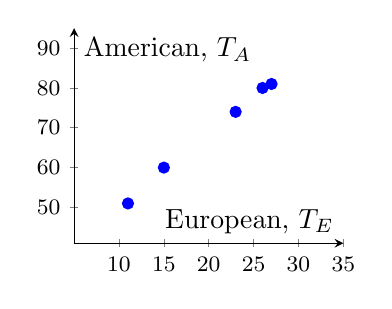
\begin{tikzpicture}
\begin{axis}[footnotesize,axis lines=middle
    ,xlabel={European, $T_E$},ylabel={American, $T_A$}
    ,xmin=5,xmax=35,ymin=41,ymax=95]
    \addplot+[only marks] coordinates {
    (26,80) (15,60) (11,51) (23,74) (27,81) };
\end{axis}
\end{tikzpicture}}%
\begin{equation*}
\begin{array}{l|rrrrr}
T_E&15&26&11&23&27\\
T_A&60&80&51&74&81
\end{array}
\end{equation*}
Example~\ref{eg:infertemp2} attempts to fit the data with the quartic polynomial
\begin{equation*}
T_A=c_1+c_2T_E+c_3T_E^2+c_4T_E^3+c_5T_E^4,
\end{equation*}
and deduced the following system of equations for the coefficients
\begin{equation*}
\begin{bmatrix} 1&15&225&3375&50625
\\1&26&676&17576&456976
\\1&11&121&1331&14641
\\1&23&529&12167&279841
\\1&27&729&19683&531441 \end{bmatrix}
\begin{bmatrix} c_1\\c_2\\c_3\\c_3\\c_4\\c_5 \end{bmatrix}
=\begin{bmatrix} 60\\80\\51\\74\\81 \end{bmatrix}.
\end{equation*}
In order to find a robust solution, here let's approximate both the matrix and the right-hand side vector because both the matrix and the vector come from real data with errors of about up to~\(\pm0.5^\circ\).

\begin{solution}
Now invoke Procedure~\ref{pro:appmat} to approximate the system of linear equations, and solve the approximate problem.
\begin{enumerate}
\item
There is a problem in approximating the matrix: the columns are of wildly different sizes.  
In contrast, our mathematical analysis treats all columns the same.  
The problem is that each column comes from different powers of temperatures.  
To avoid the problem we must scale the temperature data for the matrix.  
The simplest is to divide by a typical temperature.
That is, instead of seeking a fit in terms of powers of~\(T_E\), we seek a fit in powers of~\(T_E/20^\circ\) as \(20\)~degrees is a typical temperature in the data.
Here we fit the data with the quartic polynomial
\begin{equation*}
T_A=c_1+c_2\frac{T_E}{20} +c_3\left(\frac{T_E}{20}\right)^2+c_4\left(\frac{T_E}{20}\right)^3+c_5\left(\frac{T_E}{20}\right)^4,
\end{equation*}
which gives the following system for the coefficients \twodp
\begin{equation*}
\begin{bmatrix} 1&0.75&0.56&0.42&0.32
\\1&1.30&1.69&2.20&2.86
\\1&0.55&0.30&0.17&0.09
\\1&1.15&1.32&1.52&1.75
\\1&1.35&1.82&2.46&3.32 \end{bmatrix}
\begin{bmatrix} c_1\\c_2\\c_3\\c_3\\c_4\\c_5 \end{bmatrix}
=\begin{bmatrix} 60\\80\\51\\74\\81 \end{bmatrix}.
\end{equation*}
Now all the components of the matrix are roughly the same size, as required.

There is no need to scale the right-hand side vector as all components are all roughly the same size, they are all simply `American temperatures'. 

In script\ construct the scaled matrix and right-hand side vector with 
\begin{verbatim}
te=[15;26;11;23;27]
ta=[60;80;51;74;81]
tes=te/20
A=[ones(5,1) tes tes.^2 tes.^3 tes.^4]
\end{verbatim}
\setbox\ajrqrbox\hbox{\qrcode{% approx problem
te=[15;26;11;23;27]
ta=[60;80;51;74;81]
tes=te/20
A=[ones(5,1) tes tes.^2 tes.^3 tes.^4]
[U,S,V]=svd(A)
z=U'*ta
y=z(1:3)./diag(S(1:3,1:3))
c3=V(:,1:3)*y
}}%
\marginpar{\usebox{\ajrqrbox\\[2ex]}}%

\item Compute an \svd, \(A=\usv\), with \verb|[U,S,V]=svd(A)| to get \twodp
\begin{verbatim}
U =
  -0.16   0.64   0.20   0.72  -0.12
  -0.59  -0.13  -0.00  -0.15  -0.78
  -0.10   0.67  -0.59  -0.45   0.05
  -0.42   0.23   0.68  -0.42   0.36
  -0.66  -0.28  -0.39   0.29   0.49
S =
   7.26      0      0      0      0
      0   1.44      0      0      0
      0      0   0.21      0      0
      0      0      0   0.02      0
      0      0      0      0   0.00
V =
  -0.27   0.78  -0.49  -0.27   0.09
  -0.32   0.39   0.36   0.66  -0.42
  -0.40   0.09   0.55  -0.09   0.72
  -0.50  -0.17   0.25  -0.62  -0.52
  -0.65  -0.44  -0.51   0.32   0.14
\end{verbatim}

\item Now choose the effective rank of the matrix to be the number of singular values bigger than the error.
Here recall that the temperatures in the matrix have been divided by~\(20^\circ\).
Hence the errors of roughly~\(\pm0.5^\circ\) in each temperature becomes roughly \(\pm0.5/20=\pm0.025\) in the scaled components in the matrix.
There are three singular values larger than the error~\(0.025\), so the matrix effectively has rank three.
The two singular values less than the error~\(0.025\) are effectively zero.
That is, although it is not necessary to construct, we approximate the matrix~\(A\) by \twodp
\begin{equation*}
A_3=US_3\tr V=\begin{bmatrix} 1&0.74&0.56&0.43&0.31
\\1&1.30&1.69&2.20&2.86
\\1&0.56&0.30&0.16&0.09
\\1&1.16&1.32&1.52&1.75
\\1&1.35&1.82&2.46&3.32 \end{bmatrix}:
\end{equation*}
the differences between this and~\(A\) are only~\(\pm0.01\), so matrix~\(A_3\) is indeed close to~\(A\).

\item Solve the equations as if matrix~\(A\) has rank three.
\begin{enumerate}
\item Find \(\zv=U'\bv\) via \verb|z=U'*ta| to find
\begin{verbatim}
z =
  -146.53
    56.26
     0.41
     1.06
    -0.69
\end{verbatim}
As matrix~\(A\) has effective rank of three, we approximate the right-hand side data by neglecting the last two components in this~\zv.
That the last two components in~\zv\ are small compared to the others indicates this neglect is a reasonable approximation.

\item Find \yv\ by solving \(S\yv=\zv\) as a rank three system via \verb|y=z(1:3)./diag(S(1:3,1:3))| to find  \twodp
\begin{equation*}
\yv=(-20.19,39.15,1.95,y_4,y_5).
\end{equation*}
The smallest solution would be obtained by setting \(y_4=y_5=0\)\,.

\item Finally determine the coefficients \(\cv=V\yv\) with command \verb|c=V(:,1:3)*y| and then add arbitrary multiples of the remaining columns of~\(V\) to obtain the general solution \twodp
\begin{equation*}
\cv=
\begin{bmatrix} 35.09 \\22.50 \\12.77 \\3.99 \\-5.28 \end{bmatrix}
+y_4\begin{bmatrix} -0.27
\\0.66
\\-0.09
\\-0.62
\\0.32 \end{bmatrix}
+y_5\begin{bmatrix} 0.09
\\-0.42
\\0.72
\\-0.52
\\0.14 \end{bmatrix}.
\end{equation*}
\end{enumerate}

\item Obtain the solution with smallest coefficients by setting \(y_4=y_5=0\)\,.
This would fit the data with the quartic polynomial
{\small
\begin{equation*}
T_A=35.09+22.50\frac{T_E}{20} 
+12.77\left(\frac{T_E}{20}\right)^2
+3.99\left(\frac{T_E}{20}\right)^3
-5.28\left(\frac{T_E}{20}\right)^4.
\end{equation*}}%
But choosing the polynomial with smallest coefficients has little meaning in this application.
Surely we prefer a polynomial with fewer terms, fewer non-zero coefficients.
Surely we would prefer, say, the quadratic
\marginpar{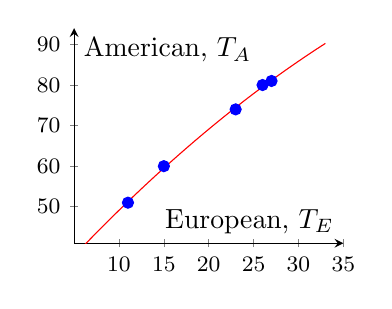
\begin{tikzpicture}
\begin{axis}[footnotesize,axis lines=middle
    ,xlabel={European, $T_E$},ylabel={American, $T_A$}
    ,xmin=5,xmax=35,ymin=41,ymax=94 ]
    \addplot+[only marks] coordinates {
    (26,80) (15,60) (11,51) (23,74) (27,81) };
%    \addplot+[domain=6:33,no marks] { 35.09+22.50*(x/20)+12.77*(x/20)^2+3.99*(x/20)^3-5.28*(x/20)^4 };
    \addplot+[domain=6:33,no marks] { 25.93+49.63*(x/20)-6.45*(x/20)^2 };
\end{axis}
\end{tikzpicture}}
\begin{equation*}
T_A=25.93+49.63\frac{T_E}{20} 
-6.45\left(\frac{T_E}{20}\right)^2,
\end{equation*}
as plotted in the margin.

In this application, let's use the freedom in~\(y_4\) and~\(y_5\) to set two of the coefficients to zero in the quartic.
Since \(c_4=3.99\) and \(c_5=-5.28\) are the smallest coefficients, and because they correspond to the highest powers in the quartic, it is natural to choose to make them both zero.
Let's redo the last step in the procedure.
\footnote{Alternatively, one could redo all the linear algebra to seek a quadratic from the outset rather than a quartic.  The two alternative answers for a quadratic are not the same, but they are nearly the same.  The small differences in the answers are because one modifies the matrix by recognising its errors, and the other does not.}

The last step in the procedure is to solve \(\tr V\cv=\yv\) for~\cv. With the last two components of~\cv\ set to zero, from the computed \svd\ this is the system of equations \twodp
\begin{equation*}
\begin{bmatrix} -0.27&-0.32&-0.40&-0.50&-0.65
\\0.78&0.39&0.09&-0.17&-0.44
\\-0.49&0.36&0.55&0.25&-0.51
\\-0.27&0.66&-0.09&-0.62&0.32
\\0.09&-0.42&0.72&-0.52&0.14 \end{bmatrix}
\begin{bmatrix} c_1\\c_2\\c_3\\0\\0 \end{bmatrix}
=\begin{bmatrix} -20.19\\39.15\\1.95\\y_4\\y_5 \end{bmatrix},
\end{equation*}
where \(y_4\) and~\(y_5\) can be anything for equally good solutions.
Considering only the first three rows of this system, and using the zeros in~\cv, this system becomes
\begin{equation*}
\begin{bmatrix} -0.27&-0.32&-0.40
\\0.78&0.39&0.09
\\-0.49&0.36&0.55 \end{bmatrix}
\begin{bmatrix} c_1\\c_2\\c_3 \end{bmatrix}
=\begin{bmatrix} -20.19\\39.15\\1.95 \end{bmatrix}.
\end{equation*}
This is a basic system of three equations for three unknowns.
Since the matrix is the first three rows and columns of~\(\tr V\) and the right-hand side is the three components of~\yv\ already computed,  we solve the equation by 
\begin{itemize}
\item  checking the \idx{condition number}, \verb|rcond(V(1:3,1:3))| is~\(0.05\) which is good, and
\item then \verb|c=V(1:3,1:3)'\y| determines the coefficients \((c_1,c_2,c_3)=(25.93,49.63,-6.45)\) \twodp.
\end{itemize}
That is, a just as good polynomial fit, consistent with errors in the data, is the simpler quadratic polynomial
\begin{equation*}
T_A=25.93+49.63\frac{T_E}{20} 
-6.45\left(\frac{T_E}{20}\right)^2,
\end{equation*}
as plotted previously in the margin.
\end{enumerate}
\end{solution}
\end{example}



\begin{quoted}{\index{Punch, John}John Punch (1639)}
\idx{Occam's razor}: Non sunt multiplicanda entia sine necessitate
[Entities must not be multiplied beyond necessity]
\end{quoted}


%\begin{example} \label{eg:} 
%Recall Examples~\ref{eg:gps2} and~\ref{eg:gps3t} showed how linear equations arise in using the \idx{Global Positioning System} to determine locations.
%Let's revisit the problem given that \gps\ data from the satellites has errors.
%\begin{comment}
%Satellite location error is typically a few metres (called ephemeris error) and satellite clock error also leads to a couple of metres error.
%Most error is in determining the travel time due to atmospheric effects and measurement errors.
%Net effect should be error of about 15\,m.
%\url{http://en.wikipedia.org/wiki/Error_analysis_for_the_Global_Positioning_System}
%Not really suitable here as measurements are too precise: better as example for over-determined system and no errors.
%\end{comment}
%\end{example}




\begin{example} \label{eg:ctscan3x3d2}
Recall that Exercise~\ref{ex:ctscan3x3d} introduced extra `diagonal' measurements into a 2D \index{CT scan}\textsc{ct}-scan.
As shown in the margin, the 2D region is divided into a \(3\times3\) grid of nine blocks.
\marginpar{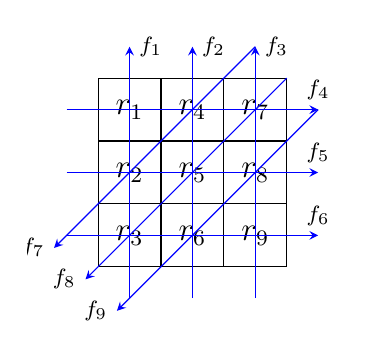
\begin{tikzpicture} 
\begin{axis}[small,font=\footnotesize
,axis equal image,axis lines=none
]
  \addplot[] coordinates {(0,0)(3,0)(3,1)(0,1)(0,2)(3,2)(3,3)(0,3)
  (0,0)(1,0)(1,3)(2,3)(2,0)(3,0)(3,3)};
  \node at (axis cs:0.5,0.5) {\large$r_3$};
  \node at (axis cs:1.5,0.5) {\large$r_6$};
  \node at (axis cs:2.5,0.5) {\large$r_9$};
  \node at (axis cs:0.5,1.5) {\large$r_2$};
  \node at (axis cs:1.5,1.5) {\large$r_5$};
  \node at (axis cs:2.5,1.5) {\large$r_8$};
  \node at (axis cs:0.5,2.5) {\large$r_1$};
  \node at (axis cs:1.5,2.5) {\large$r_4$};
  \node at (axis cs:2.5,2.5) {\large$r_7$};
  \addplot[blue,quiver={u=4,v=0},-stealth] coordinates {(-0.5,0.5)(-0.5,1.5)(-0.5,2.5)};
  \addplot[blue,quiver={u=0,v=4},-stealth] coordinates {(0.5,-0.5)(1.5,-0.5)(2.5,-0.5)};
  \addplot[blue,quiver={u=-3.2,v=-3.2},-stealth] coordinates {(3,3)(2.5,3.5)(3.5,2.5)};
  \node[right] at (axis cs:0.5,3.5) {$f_1$};
  \node[right] at (axis cs:1.5,3.5) {$f_2$};
  \node[right] at (axis cs:2.5,3.5) {$f_3$};
  \node[above] at (axis cs:3.5,0.5) {$f_6$};
  \node[above] at (axis cs:3.5,1.5) {$f_5$};
  \node[above] at (axis cs:3.5,2.5) {$f_4$};
  \node[left] at (axis cs:-0.2,-0.2) {$f_8$};
  \node[left] at (axis cs:-0.7,+0.3) {$f_7$};
  \node[left] at (axis cs:+0.3,-0.7) {$f_9$};
\end{axis}
\end{tikzpicture}}
Then measurements taken of the X-rays not absorbed along the shown nine paths: three horizontal, three vertical, and three diagonal.
Suppose the measured fractions of X-ray energy are \(\fv=(0.048\clb 0.081\clb 0.042\clb 0.020\clb 0.106\clb 0.075\clb 0.177\clb 0.181\clb 0.105)\).
Use an \svd\ to find the `grayest' transmission factors consistent with the measurements and likely errors.
\begin{verbatim}
A=[1 1 1 0 0 0 0 0 0 
 0 0 0 1 1 1 0 0 0 
 0 0 0 0 0 0 1 1 1
 1 0 0 1 0 0 1 0 0 
 0 1 0 0 1 0 0 1 0 
 0 0 1 0 0 1 0 0 1 
 0 1 0 1 0 0 0 0 0
 0 0 1 0 1 0 1 0 0
 0 0 0 0 0 1 0 1 0]
b=log([0.048
 0.081
 0.042
 0.020
 0.106
 0.075
 0.177
 0.181
 0.105])
[U,S,V]=svd(A)
z=U'*b
y=z(1:7)./diag(S(1:7,1:7))
x=V(:,1:7)*y
r=reshape(exp(A\b),3,3)
r7=reshape(exp(x),3,3)
\end{verbatim}

\begin{solution} 
Nine X-ray measurements are made through the body where \hlist f9\ denote the fraction of energy in the measurements relative to the power of the X-ray beam.
Thus we need to solve nine equations for the nine unknown transmission factors:
\begin{eqnarray*}
&&
r_1r_2r_3=f_1\,,\quad
r_4r_5r_6=f_2\,,\quad
r_7r_8r_9=f_3\,,\quad
\\&&
r_1r_4r_7=f_4\,,\quad
r_2r_5r_8=f_5\,,\quad
r_3r_6r_9=f_6\,,\quad
\\&&
r_2r_4=f_7\,,\qquad
r_3r_5r_7=f_8\,,\quad
r_6r_8=f_9\,.\quad
\end{eqnarray*}
Turn such nonlinear equations into linear equations by taking the logarithm (to any base, but here say the natural logarithm to base~\(e\)) of both sides of all equations:
\begin{equation*}
r_ir_jr_k=f_l \iff (\ln r_i)+(\ln r_j)+(\ln r_k)=(\ln f_l).
\end{equation*}
That is, letting new unknowns \(x_i=\ln r_i\) and new right-hand sides \(b_i=\ln f_i\)\,, we aim to solve a system of nine linear equations for nine unknowns:
\begin{eqnarray*}&&
x_1+x_2+x_3=b_1\,,\quad
x_4+x_5+x_6=b_2\,,\quad
x_7+x_8+x_9=b_3\,,
\\&&
x_1+x_4+x_7=b_4\,,\quad
x_2+x_5+x_8=b_5\,,\quad
x_3+x_6+x_9=b_6\,,\quad
\\&&
x_2+x_4\phantom{{}+x_4}=b_7\,,\quad
x_3+x_5+x_7=b_8\,,\quad
x_6+x_8\phantom{{}+x_4}=b_9\,.
\end{eqnarray*}
These forms the matrix-vector system \(A\xv=\bv\) for \(9\times9\) matrix
\begin{equation*}
A=\begin{bmatrix} 
 1&1&1&0&0&0&0&0&0 \\
 0&0&0&1&1&1&0&0&0 \\
 0&0&0&0&0&0&1&1&1 \\
 1&0&0&1&0&0&1&0&0 \\
 0&1&0&0&1&0&0&1&0 \\
 0&0&1&0&0&1&0&0&1 \\
 0&1&0&1&0&0&0&0&0 \\
 0&0&1&0&1&0&1&0&0 \\
 0&0&0&0&0&1&0&1&0 \end{bmatrix},\quad
 \bv=\ln\begin{bmatrix} .048
\\ .081
\\ .042
\\ .020
\\ .106
\\ .075
\\ .177
\\ .181
\\ .105 \end{bmatrix}
=\begin{bmatrix} -3.04
\\ -2.51
\\ -3.17
\\ -3.91
\\ -2.24
\\ -2.59
\\ -1.73
\\ -1.71
\\ -2.25 \end{bmatrix}.
\end{equation*}
\setbox\ajrqrbox\hbox{\qrcode{% ctscan factors
A=[1 1 1 0 0 0 0 0 0 
 0 0 0 1 1 1 0 0 0 
 0 0 0 0 0 0 1 1 1
 1 0 0 1 0 0 1 0 0 
 0 1 0 0 1 0 0 1 0 
 0 0 1 0 0 1 0 0 1 
 0 1 0 1 0 0 0 0 0
 0 0 1 0 1 0 1 0 0
 0 0 0 0 0 1 0 1 0]
b=log([0.048
 0.081
 0.042
 0.020
 0.106
 0.075
 0.177
 0.181
 0.105])
}}%
\marginpar{\usebox{\ajrqrbox\\[2ex]}}%
Implement Procedure~\ref{pro:appmat}.
\begin{enumerate}
\item Here there is no need to scale the vector~\bv\ as all entries are also the same.
There is no need to scale the matrix~\(A\) as all entries mean the same, namely simply zero or one depending upon whether  beam passes through the a pixel square.
However, the entries of~\(A\) are in error in two ways.
\begin{itemize}
\item A diagonal beam has a path through a pixel that is up to 41\% longer than horizontal or vertical beam--which is not accounted for.  Further, a beam has finite width so it will also pass through part of some off-diagonal pixels---which is not represented.
\item Similarly, a horizontal or vertical beam has finite width and may underrepresent the sides of the pixels it goes through, and/or involve parts of neighbouring pixels---neither effect is represented.
\end{itemize}
Consequently the entries in the matrix~\(A\) could easily have error of~\(0.5\).

\item Compute an \svd, \(A=\usv\), via \verb|[U,S,V]=svd(A)| \twodp
{\small
\begin{verbatim}
U =
  0.33 -0.41  0.27  0.21  0.54  0.23 -0.29  0.13 -0.41
  0.38 -0.00 -0.47  0.36 -0.45 -0.19 -0.00  0.32 -0.41
  0.33  0.41  0.27 -0.57 -0.08  0.23  0.29  0.13 -0.41
  0.33 -0.41  0.27 -0.21 -0.54  0.23 -0.29  0.13  0.41
  0.38 -0.00 -0.47 -0.36  0.45 -0.19 -0.00  0.32  0.41
  0.33  0.41  0.27  0.57  0.08  0.23  0.29  0.13  0.41
  0.23 -0.41 -0.29 -0.00  0.00  0.30  0.58 -0.52 -0.00
  0.41  0.00  0.33  0.00  0.00 -0.74 -0.00 -0.43  0.00
  0.23  0.41 -0.29 -0.00 -0.00  0.30 -0.58 -0.52  0.00
S =
  2.84     0     0     0     0     0     0     0     0
     0  2.00     0     0     0     0     0     0     0
     0     0  1.84     0     0     0     0     0     0
     0     0     0  1.73     0     0     0     0     0
     0     0     0     0  1.73     0     0     0     0
     0     0     0     0     0  1.51     0     0     0
     0     0     0     0     0     0  1.00     0     0
     0     0     0     0     0     0     0  0.51     0
     0     0     0     0     0     0     0     0  0.00
V =
  0.23 -0.41  0.29  0.00  0.00  0.30 -0.58  0.52 -0.00
  0.33 -0.41 -0.27 -0.08  0.57  0.23  0.29 -0.13 -0.41
  0.38  0.00  0.47  0.45  0.36 -0.19 -0.00 -0.32  0.41
  0.33 -0.41 -0.27  0.08 -0.57  0.23  0.29 -0.13  0.41
  0.41 -0.00 -0.33  0.00 -0.00 -0.74 -0.00  0.43 -0.00
  0.33  0.41 -0.27  0.54 -0.21  0.23 -0.29 -0.13 -0.41
  0.38  0.00  0.47 -0.45 -0.36 -0.19  0.00 -0.32 -0.41
  0.33  0.41 -0.27 -0.54  0.21  0.23 -0.29 -0.13  0.41
  0.23  0.41  0.29  0.00  0.00  0.30  0.58  0.52  0.00
\end{verbatim}
}%

\item Here choose the rank of the matrix to be effectively seven as two of the nine singular values, namely \(0.51\) and~\(0.00\), are less than about the size of the expected error, roughly~\(0.5\).

\item Use the rank seven \svd\ to solve the approximate system as in Procedure~\ref{pro:appsol}.
\begin{enumerate}
\item Find \(\zv=\tr U\bv\) via \verb|z=U'*b| to find
\begin{verbatim}
z =
  -7.63
   0.27
  -0.57
   0.42
   0.64
  -1.95
   0.64
  -0.40
  -0.01
\end{verbatim}

\item Neglect the last two rows in solving \(S_7\yv=\zv\) to find via
\verb|y=z(1:7)./diag(S(1:7,1:7))| that the first seven components of~\yv\ are
\begin{verbatim}
y =
  -2.69
   0.14
  -0.31
   0.24
   0.37
  -1.29
   0.64
\end{verbatim}
The last two components of~\yv, \(y_8\) and~\(y_9\), are free variables.

\item Obtain a particular solution to \(\tr V\xv=\yv\), the one of smallest magnitude, by setting \(y_8=y_9=0\) and determining~\xv\ from \verb|x=V(:,1:7)*y| to get the smallest solution
\begin{verbatim}
x =
  -1.53
  -0.78
  -0.67
  -1.16
  -0.05
  -1.18
  -1.16
  -1.28
  -0.68
\end{verbatim}
Obtain other equally valid solutions, in the context of the identified error in matrix~\(A\), by adding arbitrary multiples of the last two columns of~\(V\).
\end{enumerate}

\item Here we aim to make predictions from the \textsc{ct}-scan. 
The `best' solution in this application is the one with least artificial features.
The smallest magnitude~\xv\ seems to reasonably implement this criteria.
Thus use the above particular~\xv\ to determine the transmission factors, \(r_i=\exp(x_i)\).
Here use \verb|r=reshape(exp(x),3,3)| to compute and form into the \(3\times3\) array of pixels
\begin{equation*}
\begin{array}{|r|r|r|}
\hline 0.22&0.31&0.31
\\\hline 0.46&0.95&0.28
\\\hline 0.51&0.31&0.51
\\\hline
\end{array}
\end{equation*}
as illustrated  with \verb|colormap(gray),imagesc(r)|
\def\temp#1#2#3#4#5#6#7#8#9{\begin{tikzpicture}
\begin{axis}[tiny,axis equal image,colormap/blackwhite,axis lines=none]
\addplot[patch,patch type=rectangle
,point meta min={0},point meta max={1}
,table/row sep=\\,patch table with point meta={%
8 9 13 12   #1\\
4 5 9 8     #2\\
0 1 5 4     #3\\
9 10 14 13  #4\\
5 6 10 9    #5\\
1 2 6 5     #6\\
10 11 15 14 #7\\
6 7 11 10   #8\\
2 3 7 6     #9\\
}]
table[row sep=\\] {
x y \\
0 0\\% 0
1 0\\% 1
2 0\\% 2
3 0\\% 3
0 1\\% 4
1 1\\% 5
2 1\\% 6
3 1\\% 7
0 2\\% 8
1 2\\% 9
2 2\\% 10
3 2\\% 11
0 3\\% 12
1 3\\% 13
2 3\\% 14
3 3\\% 15
};
\end{axis}
\end{tikzpicture}}%
\marginpar{\temp{0.22}{0.46}{0.51}{0.31}{0.95}{0.31}{0.31}{0.28}{0.51}}
\end{enumerate}
The \textsc{ct}-scan identifies that there is a significant `hole' in the middle of the body being scanned.
\end{solution}
\end{example}




%\begin{comment}
%Maybe other application examples.
%\end{comment}










\subsection{Tikhonov regularisation}

Regularisation of poorly-posed linear equations is a widely used practical necessity.
\begin{aside} This optional extension connects to much established practice that graduates may encounter.\end{aside}
Many people have invented alternative techniques.
Many have independently re-invented techniques.
Perhaps the most common is the so-called \idx{Tikhonov regularisation}.
This section introduces and discusses Tikhonov regularisation.

\begin{quoted}{\idx{Wikipedia} (2015)}
In statistics, the method is known as ridge regression, and with multiple independent discoveries, it is also variously known as the Tikhonov--Miller method, the Phillips--Twomey method, the constrained linear inversion method, and the method of linear regularization.
\end{quoted}


\begin{definition} \label{def:Tikreg}
In seeking to solve the poorly-posed system \(A\xv=\bv\) for \(m\times n\) matrix~\(A\), a \bfidx{Tikhonov regularisation} is the system \((\tr AA+\alpha^2I_n)\xv=\tr A\bv\) for some chosen \idx{regularisation parameter} value~\(\alpha>0\).
\footnote{Some will notice that a Tikhonov regularisation is closely connected to the so-called \idx{normal equation} \(\tr AA\xv=\tr A\bv\)\,.  
Tikhonov regularisation shares some of the practical limitations of the normal equation.}
\end{definition}


\begin{example} \label{eg:}
Use \idx{Tikhonov regularisation} to solve Example~\ref{eg:2regu}:
\begin{equation*}
0.5x+0.3y=1\quad\text{and}\quad 1.1x+0.7y=-1\,,
\end{equation*}
\begin{solution} 
Here the matrix and right-hand side vector are
\begin{equation*}
A=\begin{bmatrix} 0.5&0.3\\1.1&0.7 \end{bmatrix},\quad
\bv=\begin{bmatrix} 1\\2 \end{bmatrix}.
\end{equation*}
A \idx{Tikhonov regularisation}, \((\tr AA+\alpha^2I_n)\xv=\tr A\bv\)\,, is then the system
\begin{equation*}
\begin{bmatrix} 1.46+\alpha^2&0.92\\0.92&0.58+\alpha^2 \end{bmatrix}\xv=\begin{bmatrix} 2.7\\1.7 \end{bmatrix}.
\end{equation*}
Choose regularisation parameter~\(\alpha\) to be roughly the error: here the error is~\(\pm0.05\) so let's choose \(\alpha=0.1\) (\(\alpha^2=0.01\)).
Enter into \script\ with
\begin{verbatim}
A=[0.5 0.3;1.1 0.7]
b=[1.0;2.0]
At=(A'*A+0.01*eye(2))
bt=A'*b
rcondA=rcond(At)
x=At\bt
\end{verbatim}
\setbox\ajrqrbox\hbox{\qrcode{% 2x2 Tikhonov
A=[0.5 0.3;1.1 0.7]
b=[1.0;2.0]
At=(A'*A+0.01*eye(2))
bt=A'*b
rcondA=rcond(At)
x=At\slosh bt
}}%
\marginpar{\usebox{\ajrqrbox\\[2ex]}}%
to find the Tikhonov regularised solution is \(\xv=(1.39,0.72)\).%
\footnote{Interestingly, \(\texttt{rcond}=0.003\) for the Tikhonov system which is worse than \(\texttt{rcond}(A)\).  The regularisation only works because pre-multiplying by~\(\tr A\) puts both sides in the row space of~\(A\) (except for numerical error and the small~\(\alpha^2I\) factor).}
This solution is reasonably close to the smallest solution found by the \svd\ which is~\((1.32,0.83)\).
However, Tikhonov regularisation gives no hint of the reasonable general solutions found by the \svd\ approach of Example~\ref{eg:2regu}.

Change the regularisation parameter to \(\alpha=0.01\) and \(\alpha=1\) and see that both degrade the Tikhonov solution.
\end{solution}
\end{example}



Do not apply \idx{Tikhonov regularisation} blindly as it does introduce biases. 
The following example illustrates the bias.

\begin{example} \label{eg:}
Recall the example at the start of Section~\ref{sec:mmctp} where my scales variously reported my weight in kg as~\(84.8\), \(84.1\), \(84.7\) and~\(84.4\)\,.  
To best estimate my weight~\(x\) we rewrote the problem in matrix-vector form
\begin{equation*}
Ax=\bv\,,\quad\text{namely }
\begin{bmatrix} 1\\1\\1\\1 \end{bmatrix}x
=\begin{bmatrix} 84.8\\84.1\\84.7\\84.4 \end{bmatrix}.
\end{equation*}
A Tikhonov regularisation of this inconsistent system is
\begin{equation*}
\left(\begin{bmatrix} 1&1&1&1 \end{bmatrix}\begin{bmatrix} 1\\1\\1\\1 \end{bmatrix}+\alpha^2\right)x
=\begin{bmatrix} 1&1&1&1 \end{bmatrix}\begin{bmatrix} 84.8\\84.1\\84.7\\84.4 \end{bmatrix}.
\end{equation*}
That is, \((4+\alpha^2)x=338\)\,kg with solution \(x=84.5/(1+\alpha^2/4)\)\,kg.
This Tikhonov answer is biased because it is systematically below the average~\(84.5\)\,kg.
For small Tikhonov parameter~\(\alpha\) it is only a small bias, but even so such a bias is unpleasant.
\end{example}



\begin{example} \label{eg:}
Use \idx{Tikhonov regularisation} to solve \(A\xv=\bv\) for the matrix and vector of Example~\ref{eg:3regmata}.
\begin{solution} 
Here the matrix and right-hand side vector are
\begin{equation*}
A=\begin{bmatrix} -0.2&-0.6&1.8
\\ 0.0&0.2&-0.4
\\ -0.3&0.7&0.3 \end{bmatrix}, \quad
\bv=\begin{bmatrix} -0.5
\\ 0.1
\\ -0.2
 \end{bmatrix}.
\end{equation*}
A \idx{Tikhonov regularisation}, \((\tr AA+\alpha^2I_n)\xv=\tr A\bv\)\,, is then the system
\begin{equation*}
\begin{bmatrix} 0.13+\alpha^2&-0.09&-0.45
\\-0.09&0.89+\alpha^2 &-0.95
\\-0.45&-0.95&3.49+\alpha^2\end{bmatrix}\xv
=\begin{bmatrix} 0.16\\0.18\\-1.00 \end{bmatrix}.
\end{equation*}
Choose regularisation parameter~\(\alpha\) to be roughly the error: here the error is~\(\pm0.05\) so let's choose \(\alpha=0.1\) (\(\alpha^2=0.01\)).
Enter into and solve with \script\ via
\begin{verbatim}
A=[-0.2 -0.6 1.8
   0.0 0.2 -0.4
  -0.3 0.7 0.3 ]
b=[-0.5;0.1;-0.2]
At=(A'*A+0.01*eye(3))
bt=A'*b
rcondA=rcond(At)
x=At\bt
\end{verbatim}
\setbox\ajrqrbox\hbox{\qrcode{% 3x3 Tikhonov
A=[-0.2 -0.6 1.8
   0.0 0.2 -0.4
  -0.3 0.7 0.3 ]
b=[-0.5;0.1;-0.2]
At=(A'*A+0.01*eye(3))
bt=A'*b
rcondA=rcond(At)
x=At\slosh bt
}}%
\marginpar{\usebox{\ajrqrbox\\[2ex]}}%
which then finds the Tikhonov regularised solution is \(\xv=(0.10,-0.11,-0.30)\).
To two decimal places this is the same as the smallest solution found by an \svd.
However, Tikhonov regularisation gives no hint of the reasonable general solutions found by the \svd\ approach of Example~\ref{eg:3regmata}.
\end{solution}
\end{example}








\begin{theorem}[Tikhonov regularisation] \label{thm:Tikreg}
Solving the \idx{Tikhonov regularisation}, with parameter~\(\alpha\), of \(A\xv=\bv\) is equivalent to finding the \index{smallest solution}smallest, \idx{least square}, solution of the system \(\tilde A\xv=\bv\) where  
%\begin{itemize}
%\item 
the matrix~\(\tilde A\) is obtained from~\(A\) by replacing each of its non-zero \idx{singular value}s~\(\sigma_i\) by \(\tilde\sigma_i:=\sigma_i+\alpha^2/\sigma_i\)\,.
%, and
%\item the vector~\(\tilde\bv\) is the orthogonal projection of~\(\bv\) onto the column space~\AA\ of~\(A\),  \(\tilde\bv=\proj_\AA\bv\)\,.
%\end{itemize}
\end{theorem}

\begin{proof} 
Let \(m\times n\) matrix~\(A\) have \svd\ \(A=\usv\).
First, the left-hand side matrix in a Tikhonov regularisation is
\begin{eqnarray*}
\tr AA+\alpha^2I_n
&=&\tr{(\usv)}\usv+\alpha^2I_nV\tr V
\\&=&V\tr S\tr U\usv+\alpha^2VI_n\tr V
\\&=&V\tr SS\tr V+V(\alpha^2I_n)\tr V
\\&=&V(\tr SS+\alpha^2I_n)\tr V,
\end{eqnarray*}
whereas the right-hand side is \(\tr A\bv =\tr{(\usv)}\bv =V\tr S\tr U\bv\)\,.
Corresponding to the variables used in previous procedures, let \(\zv=\tr U\bv\in\RR^m\) and as yet unknown \(\yv=\tr V\xv\in\RR^n\). 
Then equating the above two sides, and premultiplying by the orthogonal~\(\tr V\), means the Tikhonov regularisation is equivalent to solving \((\tr SS+\alpha^2I_n)\yv=\tr S\zv\) for~\yv.

Second, suppose \(\rank A=r\) so that the singular value matrix
\begin{equation*}
S=\begin{bmatrix} \begin{matrix} \sigma_1&\cdots&0\\
\vdots&\ddots&\vdots\\
0&\cdots&\sigma_r \end{matrix} & 
O_{r\times (n-r)}\\\,\\
O_{(m-r)\times r}&O_{(m-r)\times (n-r)}\end{bmatrix}
\end{equation*}
(where the bottom right zero block contains all the zero singular values).
Consequently, the equivalent Tikhonov regularisation, \((\tr SS+\alpha^2I_n)\yv=\tr S\zv\), becomes
\begin{equation*}
\begin{bmatrix} \begin{matrix} \sigma_1^2+\alpha^2&\cdots&0\\
\vdots&\ddots&\vdots\\
0&\cdots&\sigma_r^2+\alpha^2 \end{matrix} & 
O_{r\times (n-r)}\\\,\\
O_{(n-r)\times r}&\alpha^2I_{n-r}\end{bmatrix}\yv
=\begin{bmatrix} \sigma_1z_1\\\vdots\\\sigma_rz_r\\\,\\\ov_{n-r} \end{bmatrix}.
\end{equation*}
Dividing each of the first \(r\)~rows by the corresponding non-zero singular value, \hlist\sigma r, the equivalent system is
\begin{equation*}
\begin{bmatrix} \begin{matrix} \sigma_1+\alpha^2/\sigma_1&\cdots&0\\
\vdots&\ddots&\vdots\\
0&\cdots&\sigma_r+\alpha^2/\sigma_r \end{matrix} & 
O_{r\times (n-r)}\\\,\\
O_{(n-r)\times r}&\alpha^2I_{n-r}\end{bmatrix}\yv
=\begin{bmatrix} z_1\\\vdots\\z_r\\\,\\\ov_{n-r} \end{bmatrix},
\end{equation*}
with solution 
\begin{itemize}
\item \(y_i=z_i/(\sigma_i+\alpha^2/\sigma_i)\) for \(i=1,\ldots,r\)\,, and
\item \(y_i=0\) for \(i=r+1,\ldots,n\) (since \(\alpha^2>0\)).
\end{itemize}
This establishes that solving the Tikhonov system is equivalent to performing the \svd\ Procedure~\ref{pro:appsol} for the least square solution to \(A\xv=\bv\) but with two changes in Step~\ref{as:a2}:
\begin{itemize}
\item for $i=1,\ldots,r$ divide by \(\tilde\sigma_i:=\sigma_i+\alpha^2/\sigma_i\) instead of the true singular value~\(\sigma_i\) (the margin plots \(\tilde\sigma\) versus~\(\sigma\)), and
\item for $i=r+1,\ldots,n$ set \(y_i=0\) to obtain the smallest possible solution (Theorem~\ref{thm:smallsoln}).
\end{itemize}
Thus \idx{Tikhonov regularisation} of \(A\xv=\bv\) is equivalent to finding the smallest, {least square}, solution of the system \(\tilde A\xv=\bv\)\,.
\end{proof}


There is another reason to be careful when using Tikhonov regularisation. 
Yes, it gives a nice, neat, unique solution.
However, it does not hint that there may be an infinite number of equally good nearby solutions (as found through Procedure~\ref{pro:appmat}).
Among those equally good nearby solutions may be ones that you prefer in your application.

\Needspace{5\baselineskip}
\paragraph{Choose a good regularisation parameter}
\begin{itemize}
\item One strategy to choose the \idx{regularisation parameter}~\(\alpha\) is that the effective change in the matrix, from~\(A\) to~\(\tilde A\), should be about the size of errors expected in~\(A\).
\footnote{This strategic choice is sometimes called the \idx{discrepancy principle} \cite[\S7]{Kress2015}.}
Since changes in the matrix are largely measured by the \idx{singular value}s we need to consider the relation between \(\tilde\sigma=\sigma+\alpha^2/\sigma\) and~\(\sigma\).
\marginpar{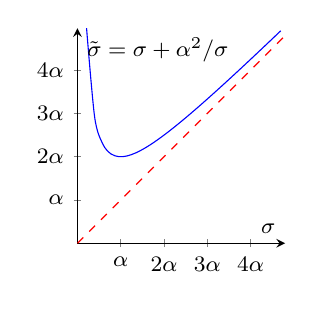
\begin{tikzpicture}
\begin{axis}[footnotesize,font=\footnotesize
  ,axis lines=middle,ymin=0,xmin=0,axis equal image
  ,xlabel={$\sigma$},ylabel={$\tilde\sigma=\sigma+\alpha^2/\sigma$}
  ,xticklabel={$\ifcase\tick\or\or2\or3\or4\fi\alpha$}
  ,yticklabel={$\ifcase\tick\or\or2\or3\or4\fi\alpha$}
  ]
\addplot[blue,domain=0.21:4.7,smooth] {x+1/x};
\addplot[red,dashed,domain=0:4.8] {x};
\end{axis}
\end{tikzpicture}}
From the marginal graph the small singular values are changed by a lot, but these are the ones for which we want~\(\tilde\sigma\) large in order give a `least square' approximation.
Significantly, the marginal graph also shows that singular values larger than~\(\alpha\) change by less than~\(\alpha\).
Thus the parameter~\(\alpha\) should not be much larger than the expected error in the elements of the matrix~\(A\).

\item Another consideration is the effect of regularisation upon errors in the right-hand side vector.
The condition number of~\(A\) may be very bad.
However, as the marginal graph shows the smallest~\(\tilde\sigma\geq2\alpha\).
Thus, in the regularised system the \idx{condition number} of the effective matrix~\(\tilde A\) is approximately~\(\sigma_1/(2\alpha)\).
We need to choose the regularisation parameter~\(\alpha\) large enough so that \(\frac{\sigma_1}{2\alpha}\times\)(relative error in~\bv) is an acceptable \idx{relative error} in the solution~\xv\ (Theorem~\ref{thm:erramp}).
It is only when the \idx{regularisation parameter}~\(\alpha\) is big enough that the regularisation will be effective in finding a \idx{least square} approximation. 

\end{itemize}








\subsection{Exercises}



\begin{exercise} \label{ex:errmats} 
For each of the following matrices, say~\(A\), and right-hand side vectors, say~\(\bv_1\),
solve \(A\xv=\bv_1\)\,.
But suppose the matrix entries come from experiments and are only known to within errors~\(\pm0.05\).
Thus within experimental error the given matrices~\(A'\) and~\(A''\) may be the `true' matrix~\(A\).
Solve \(A'\xv'=\bv_1\) and \(A''\xv''=\bv_1\) and comment on the results.
Finally, use an \svd\ to find a general solution consistent with the error in the matrix.
%\begin{verbatim} A brutal search for such problems
%format bank
%n=2
%for k=1:999
%  A=0+round(randn(n)*10)/10; 
%  if(min(svd(A))<0.02)&(rcond(A)>0.005)
%  A=A
%  b=0+round(A*randn(n,1)*10)/10, x=(A\b)'
%  Ad=A+round(rand(n)*9-4.5)/100, xd=(Ad\b)'
%  Add=A+round(rand(n)*9-4.5)/100, xdd=(Add\b)'
%  [U,S,V]=svd(A); S=diag(S), k=sum(S>0.05)
%  z=U(:,1:k)'*b; y=z./S(1:k); xsmall=(V(:,1:k)*y)'  
%  Vker=V(:,k+1:end)'
%  break,end
%end
%\end{verbatim}

\begin{enumerate} \raggedright
\item \(\eAii=\begin{bmatrix} -1.3&-0.4\\0.7&0.2 \end{bmatrix}\),
\(\bv_{\arabic{enumii}}=\begin{bmatrix} 2.4\\-1.3 \end{bmatrix}\), 
\(\eAii'=\begin{bmatrix} -1.27&-0.43\\0.71&0.19 \end{bmatrix}\),
\(\eAii''=\begin{bmatrix} -1.27&-0.38\\0.66&0.22 \end{bmatrix}\).
\answer{\(\xv=(-2.00,0.50)\),
\(\xv'=(-1.61,-0.83)\),
\(\xv''=(-1.19,-2.34)\),
\(\xv=(-1.69,-0.51)+t(0.29,-0.96)\) \twodp.}

\item \(\eAii=\begin{bmatrix} -1.8&-1.1
\\-0.2&-0.1 \end{bmatrix}\),
\(\bv_{\arabic{enumii}}=\begin{bmatrix} -0.7
\\-0.1 \end{bmatrix}\), 
\(\eAii'=\begin{bmatrix} -1.81&-1.13
\\-0.24&-0.12 \end{bmatrix}\),
\(\eAii''=\begin{bmatrix} -1.81&-1.13
\\-0.18&-0.1 \end{bmatrix}\).
\answer{\(\xv=(1.0,-1.0)\),
\(\xv'=(0.54,-0.24)\),
\(\xv''=(1.92,-2.46)\),
\(\xv=(0.28,0.17)+t(-0.52,0.85)\) \twodp.}

\item \(\eAii=\begin{bmatrix} 0.8&-0.1
\\-1.0&0.1 \end{bmatrix}\),
\(\bv_{\arabic{enumii}}=\begin{bmatrix} 0.2
\\-0.3 \end{bmatrix}\), 
\(\eAii'=\begin{bmatrix} 0.81&-0.07
\\-1.01&0.06 \end{bmatrix}\),
\(\eAii''=\begin{bmatrix} 0.79&-0.08
\\-1.03&0.09 \end{bmatrix}\).
\answer{\(\xv=(0.5,2.0)\),
\(\xv'=(0.41,1.86)\),
\(\xv''=(0.53,2.74)\),
\(\xv=(0.28,-0.03)+t(-0.11,-0.99)\) \twodp.}

\item \(\eAii=\begin{bmatrix} 0.0&0.5&-0.5
\\0.6&0.5&0.9
\\0.6&1.3&0.0 \end{bmatrix}\),
\(\bv_{\arabic{enumii}}=\begin{bmatrix} -1.4
\\0.4
\\-1.9 \end{bmatrix}\), 
\(\eAii'=\begin{bmatrix} -0.02&0.49&-0.49
\\0.58&0.54&0.9
\\0.61&1.34&-0.02 \end{bmatrix}\),
\(\eAii''=\begin{bmatrix} -0.04&0.52&-0.48
\\0.64&0.52&0.87
\\0.57&1.33&0.04 \end{bmatrix}\).
\answer{\(\xv=(1.6,-2.2,0.6)\),
\(\xv'=(1.31,-2.0,0.8)\),
\(\xv''=(-0.28,-1.35,1.47)\),
\(\xv=(-0.09,-1.43,1.32)+t(0.85,-0.39,-0.36)\) \twodp.}

\item \(\eAii=\begin{bmatrix} 0.6&-0.8&-0.2
\\-0.9&1.0&1.2
\\-0.9&0.9&1.4 \end{bmatrix}\),
\(\bv_{\arabic{enumii}}=\begin{bmatrix} 1.1
\\-3.7
\\-4.1 \end{bmatrix}\), 
\(\eAii'=\begin{bmatrix} 0.57&-0.78&-0.23
\\-0.91&0.99&1.22
\\-0.93&0.9&1.39 \end{bmatrix}\),
\(\eAii''=\begin{bmatrix} 0.56&-0.77&-0.21
\\-0.87&1.01&1.22
\\-0.87&0.9&1.39 \end{bmatrix}\).
\answer{\(\xv=(-0.33,-1.0,-2.5)\),
\(\xv'=(0.84,-0.11,-2.31)\),
\(\xv''=(1.54,0.29,-2.17)\),
\(\xv=(0.65,-0.32,-2.32)+t(-0.81,-0.57,-0.15)\) \twodp.}

\item \(\eAii=\begin{bmatrix} 0.1&-1.0&0.0
\\2.1&-0.2&-0.5
\\0.0&-1.6&0.0 \end{bmatrix}\),
\(\bv_{\arabic{enumii}}=\begin{bmatrix} -0.2
\\1.6
\\-0.5 \end{bmatrix}\), 
\(\eAii'=\begin{bmatrix} 0.1&-0.98&-0.04
\\2.11&-0.17&-0.47
\\-0.04&-1.62&-0.01 \end{bmatrix}\),
\(\eAii''=\begin{bmatrix} 0.14&-0.96&0.01
\\2.13&-0.23&-0.47
\\0.0&-1.57&-0.02 \end{bmatrix}\).
\answer{\(\xv=(1.12,0.31,1.4)\),
\(\xv'=(0.59,0.3,-0.84)\),
\(\xv''=(0.77,0.32,-0.08)\),
\(\xv=(0.75,0.3,-0.18)+t(-0.23,-0.01,-0.97)\) \twodp.}

\item \(\eAii=\begin{bmatrix} 1.0&-0.3&0.3&-0.4
\\1.8&0.5&0.1&0.2
\\0.2&-0.3&1.3&-0.6
\\0.0&0.5&1.2&0.0 \end{bmatrix}\),
\(\bv_{\arabic{enumii}}=\begin{bmatrix} 2.0
\\1.6
\\1.4
\\-0.2 \end{bmatrix}\), 
\(\eAii'=\begin{bmatrix} 0.98&-0.3&0.31&-0.44
\\1.8&0.54&0.06&0.21
\\0.24&-0.33&1.27&-0.58
\\0.01&0.52&1.23&-0.01 \end{bmatrix}\),
\(\eAii''=\begin{bmatrix} 1.03&-0.32&0.33&-0.36
\\1.82&0.49&0.08&0.16
\\0.2&-0.31&1.33&-0.64
\\0.0&0.49&1.22&0.0 \end{bmatrix}\).
\answer{\(\xv=(1.21,-0.53,0.06,-1.54)\),
\(\xv'=(1.25,-0.79,0.15,-1.11)\),
\(\xv''=(1.28,-1.56,0.46,-0.07)\),
\(\xv=(1.26,-1.0,0.25,-0.9)+t(0.06,-0.57,0.23,0.79)\) \twodp.}

\item \(\eAii=\begin{bmatrix} -0.9&-0.5&-0.3&-0.4
\\-0.1&0.1&-0.2&0.8
\\-1.0&0.4&-1.1&0.6
\\1.0&2.2&-1.0&-0.1 \end{bmatrix}\),
\(\bv_{\arabic{enumii}}=\begin{bmatrix} 0.4
\\0.3
\\0.2
\\-2.0 \end{bmatrix}\), 
\(\eAii'=\begin{bmatrix} -0.88&-0.52&-0.33&-0.41
\\-0.11&0.13&-0.17&0.78
\\-0.96&0.44&-1.12&0.61
\\0.98&2.19&-0.99&-0.13 \end{bmatrix}\),
\(\eAii''=\begin{bmatrix} -0.86&-0.49&-0.29&-0.37
\\-0.06&0.14&-0.18&0.83
\\-0.96&0.38&-1.11&0.58
\\1.01&2.21&-1.04&-0.13 \end{bmatrix}\).
\answer{\(\xv=(-0.76,-0.23,0.69,0.48)\),
\(\xv'=(-1.36,0.33,1.35,0.43)\),
\(\xv''=(-0.09,-0.92,-0.17,0.47)\),
\(\xv=(-0.38,-0.63,0.2,0.47)+t(0.52,-0.54,-0.67,-0.02)\) \twodp.}

\end{enumerate}
\end{exercise}



\begin{exercise} \label{ex:hilb7} 
Recall Example~\ref{eg:hilb5} explores the effective rank of the \(5\times5\) \idx{Hilbert matrix} depending upon a supposed level of error.
Similarly, explore the effective rank of the \(7\times7\) \idx{Hilbert matrix} (\verb|hilb(7)| in \script) depending upon supposed levels of error in the matrix.
What levels of error in the components would give what effective rank of the matrix?
\answer{rank one, \(1>e>0.3\);
two,~\(0.3>e>0.02\);
three,~\(0.02>e>0.001\);
four,~\(0.001>e>3\cdot10^{-5}\);
five,~\(3\cdot10^{-5}>e>5\times 10^{-7}\);
six,~\(5\times 10^{-7}>e>3\cdot10^{-9}\);
seven,~\(3\times 10^{-9}>e\).}
\end{exercise}




% Could do GPS exercises analogous to Exercise~\ref{ex:gps3t}
% or University ranking exercise





\begin{exercise} \label{ex:orb4Periods2} 
Recall Exercise~\ref{ex:orb4Periods} considered the inner four planets in the solar system.
The exercise fitted fit a quadratic polynomial to the orbital period \(T=c_1+c_2R+c_3R^2\) as a function of distance~\(R\) using the data of Table~\ref{tbl:orb4Periods}.
In view of the bad condition number, \(\verb|rcond|=6\cdot10^{-6}\), revisit the task with the more powerful techniques of this section.
Use the data for Mercury, Venus and Earth to fit the quadratic and predict the period for Mars.
Discuss how the bad condition number is due to the failure in Exercise~\ref{ex:orb4Periods} of scaling the data in the matrix.
%\begin{verbatim}
%t=[87.97;224.70;365.26]
%r=[57.91;108.21;149.60]
%rs=r/100
%A=[ones(3,1) rs rs.^2]
%rcond(A)
%c=A\t
%tmars=c(1)+c(2)*227.94/100+c(3)*(227.94/100)^2
%relerr=tmars/686.97-1
%\end{verbatim}
\end{exercise}



\begin{exercise} \label{ex:} 
Recall Exercise~\ref{ex:ctscan4x4d} used a \(4\times4\) grid of pixels in the \idx{computed tomography} of a \textsc{ct}-scan.
Redo this exercise recognising that the entries in matrix~\(A\) have errors up to roughly~\(0.5\).
Discuss any change in the prediction.
\answer{The matrix has effective rank of eleven.  
Pixel ten is still the most absorbing.  
The corner pixels are the most affected.}
\end{exercise}




\begin{exercise} \label{ex:} 
Reconsider each of the matrix-vector systems you explored in Exercise~\ref{ex:errmats}.
Also solve each system using \idx{Tikhonov regularisation}; for example, in the first system solve \(A\xv=\bv_1\)\,, \(A'\xv'=\bv_1\) and \(A''\xv''=\bv_1\).
Discuss why \(\xv\), \(\xv'\) and~\(\xv''\) are all reasonably close to the smallest solution of those obtained via an \svd.
\end{exercise}




\begin{exercise} \label{ex:} 
Recall that Example~\ref{eg:hilb5} explores the effective rank of the \(5\times5\) \idx{Hilbert matrix} depending upon a supposed level of error.
Here do the alternative and solve the system \(A\xv=\vec 1\) via \idx{Tikhonov regularisation} using a wide range of various regularisation parameters~\(\alpha\).
Comment on the relation between the solutions obtained for various~\(\alpha\) and those obtained in the example for the various presumed error---perhaps plot the components of~\xv\ versus parameter~\(\alpha\) (on a log-log plot).
\end{exercise}




\begin{exercise} \label{ex:} 
Recall Example~\ref{eg:ctscan3x3d2} used a \(3\times3\) grid of pixels in the \idx{computed tomography} of a \textsc{ct}-scan.
Redo this example with \idx{Tikhonov regularisation} recognising that the entries in matrix~\(A\) have errors up to roughly~\(0.5\).
Discuss the relation between the solution of Example~\ref{eg:ctscan3x3d2} that of \idx{Tikhonov regularisation}.
\end{exercise}




\begin{exercise} \label{ex:} 
Recall Exercise~\ref{ex:ctscan4x4d} used a \(4\times4\) grid of pixels in the \idx{computed tomography} of a \textsc{ct}-scan.
Redo this exercise with \idx{Tikhonov regularisation} recognising that the entries in matrix~\(A\) have errors up to roughly~\(0.5\).
Discuss any change in the prediction.
\end{exercise}








\begin{comment}%{ED498555.pdf}
why, what caused X?
how did X occur?
what-if? what-if-not?
how does X compare with Y?
what is the evidence for X?
why is X important?
\end{comment}






\begin{comment}
Possible extensions of this chapter include Frobenius norm.  
Possibly link to polar decomposition (Higham86) 
see closestOrthogonalMatrix.png

\begin{exercise} \label{ex:} 
Prove that for any square matrix~\(A\) with \svd\ \(\usv\), a closest orthogonal matrix to~\(A\) is~\(U\tr V\) ??
\begin{center}
\TwoD1101
\TwoD{0.89443}{0.44721}{0.44721}{1.34164}%H or R
\TwoD{0.89443}{0.44721}{-0.44721}{0.89443}%U or Q
\end{center}
\end{exercise}
\end{comment}


